

\section{Andere Datenstrukturen und Annotation}
\begin{frame}[fragile]{Annotation und Erschließung}

\begin{columns}
\metroset{block=fill}
\column{0.45\textwidth}

\begin{alertblock}{Annotation zur Erschließung}
\small 
irgendwelche (Meta-)Daten sammeln (\emph{curation-driven}) vs. gezielt spezifische Daten verfügbarmachen (\emph{research-driven})
\bigskip

Markup = Annotation = Kodierung 
\end{alertblock}

\column{0.55\textwidth}
\begin{exampleblock}{Was ist Annotation?}
\begin{itemize}\footnotesize
\item Metadaten
\item Bedeutung kodieren 
\item Strukturmerkmale, Wissen und Erkenntnisse (implizite Strukturen) für die Maschine explizit machen für Verarbeitung und Nachnutzung. 
\item \textbf{Im Druckwesen:} inhaltliche Korrektur und typographische Anweisungen (Druckvorbereitung) 
\item \textbf{Computer:} Einbettung von Markup in elektronische Dokumente (log. Struktur beschreiben)
\end{itemize}
\end{exampleblock}

\end{columns}

\end{frame}


%-----------------------------------------------------
\begin{frame}{Markup / Annotation}
\metroset{block=fill}

\begin{exampleblock}{Annotation = `Auszeichnung' = Mark-up}
\begin{quote}
Eine Auszeichnungssprache (\emph{markup language}, abgekürzt ML) ist eine maschinenlesbare Sprache für die Gliederung und Formatierung von Texten und anderen Daten. Der bekannteste Vertreter ist die \emph{Hypertext Markup Language} (HTML), die Kernsprache des World Wide Webs.

Mit Auszeichnungssprachen werden Eigenschaften, Zugehörigkeiten und Darstellungsformen von Abschnitten eines Textes (Zeichen, Wörtern, Absätzen usw. -- ``Elementen'') oder einer Datenmenge beschrieben. Dies geschieht in der Regel, indem sie mit \emph{Tags} markiert werden.\punkti mit der \emph{Standard Generalized Markup Language} (SGML) empfohlene ``Trennung von Struktur und Darstellung''. (\href{https://de.wikipedia.org/wiki/Auszeichnungssprache}{Wikipedia})
\end{quote}
\end{exampleblock}
\end{frame}
%-----------------------------------------------------

\begin{frame}{Praktische Tipps}
 Tools zum `Switchen' zwischen Markups/Markdown: 
 z.B.~ \href{https://pandoc.org/}{Pandoc} oder \href{http://oxgarage.tei-c.org}{OxGarage} (TEI-Fokus). \\

Binäre Dokumentenformate  wie \texttt{.doc, .pdf, .dvi} (\TeX{}-Ausgabeformat) $\neq$ Auszeichnungssprachen. \texttt{.docx} ist eigentlich ein \texttt{.zip} mit XML-Daten, die man, wenn man es entzippt, auch anschauen und bearbeiten kann (aber etwas unübersichtlich). Daher ist es mit Oxgarage und Pandoc relativ leicht transformierbar.

Ziel: \textbf{Implizites explizieren} $\to$ für nicht in Tabellenform vorliegende bzw. nicht sinnvoll darinabbildbare Daten, wie z.B. Text
\end{frame}


%-------------------------------


\section{Annotation im Alltag}
%---------------------------------------------
\begin{frame}{\href{https://de.wikipedia.org/wiki/Standard_Generalized_Markup_Language}{SGML}}

\begin{itemize}
    \item \bg{alert}{white}{Trennung von Inhalt und Darstellung}
    \item \bg{alert}{white}{Wie XML: Metasprache} \textasciitilde
HTML und XML (Nachfolger von SGML genannt $\to$  SGML-basierend) 
    \item Metasprache zur Definition von Auszeichnungssprachen für Dokumente 
    \item \emph{Genormte Verallgemeinerte Auszeichnungssprache} (en: \textbf{Standard Generalized Markup Language}
\end{itemize}

\bgupper{w3schools}{black}{.sgml}

\end{frame}





%-----------------------------------------------------
\begin{frame}[fragile]{\href{https://de.wikipedia.org/wiki/Rich_Text_Format}{RTF}}
\bg{alert}{white}{Rich Text Format}
\begin{columns}
\column{0.45\textwidth}
\begin{itemize}
    \item Microsoft 1987 \item Austauschformat zwischen Textverarbeitungsprogrammen (versch. Hersteller und Betriebssysteme). \item enthält im Gegensatz zu `plain text' Markup zur Textformatierung
\end{itemize}
\column{0.45\textwidth}
\bgupper{w3schools}{black}{.rtf}\\
\footnotesize
\begin{verbatim}
{\rtf1
Guten Tag!
\line
{\i Dies} ist \b{\i ein
\i0 formatierter \b0Text}.
\par
\b Das \b0Ende.
} 
\end{verbatim}\normalsize
\end{columns}

\end{frame}

%-----------------------------------------------------
\begin{frame}[fragile]{\href{https://de.wikipedia.org/wiki/JavaScript_Object_Notation}{JavaScript Object Notation}}
\begin{columns}
\column{0.55\textwidth}
\begin{itemize}\footnotesize
    \item ausgesprochen wie `Jason' \item kompaktes Datenformat \item menschen- und maschinenlesbar \item key-value-Paare \item Verschachtelung
\end{itemize}

\bg{alert}{white}{Alternative zu XML? Unterschiede}\\
\begin{itemize}\footnotesize
    \item XML = Struktur-beschreibend, JSON = Syntax-Konvention (nicht deklarativ) \item JSON: Definition von Instanzen strukturierter Daten
\end{itemize}

\bg{alert}{white}{Fazit}~ JSON im Vorteil, wo simple key-value-Paare (\textbf{`Einfachheit'}). XML hat und erlaubt mehr \textbf{Komplexität}.
\bg{w3schools}{white}{XML = Auszeichnungssprache}~\\
\bg{w3schools}{white}{JSON = Datenaustauschformat}~


\column{0.5\textwidth}
\bgupper{w3schools}{black}{.json}
\footnotesize
\begin{verbatim}
{
  "Herausgeber": "Xema",
  "Nummer": "1234-5678-9012-3456",
  "Inhaber":
  {
    "Name": "Mustermann",
    "Vorname": "Max",
    "maennlich": true,
    "Hobbys": ["Reiten", "Golfen", "Lesen"],
    "Alter": 42,
    "Kinder": [],
    "Partner": null
  }
}
\end{verbatim}\normalsize
\end{columns}


\end{frame}


%-------------------------------
\begin{frame}[fragile]{\LaTeX}

\begin{columns}
\column{0.5\textwidth}\small 
\begin{itemize}
    \item \bg{w3schools}{white}{.tex} Textsatz mit \TeX{} durch Lamport-Makros (= `Shortcuts)
\item \LaTeX{} liest Makros (mit sprechenden Namen) ein -- in der `Produktion' entsteht die `Illusion' rein deskriptiver Auszeichnung, im Hintergrund sind dies allerdings nur Stellvertreter für die komplexe prozedurale Sprache \TeX . \item prozedural vs. präsentational: \textbf{WYIWYG} (\emph{what you see is what you get}, z.B. Word) vs. \textbf{WYSIWYM} (\emph{what you see is what you mean}) \LaTeX{}-Editoren) 
\end{itemize}
\column{0.5\textwidth}
\footnotesize
Befehle unten ohne spaces vor der Klammer \\
\mycommand{\textit{Italic}}{\textit{Italic} (darst.)}
\mycommand{\emph{Italic}}{\textit{Italic} (beschr. / semant.)}
\mycommand{\textbf{Bold}}{\textbf{Bold}}
\mycommand{\section{Titel}}{Überschrift 1}
\mycommand{\subsection{Titel}}{usw.}
\mycommand{\href{http://a.com}{Link}}{\href{https://www.latex-project.org/latex3/}{`hidden' Link}}
\mycommand{\includegraphics{bla.png}}{Bild}
\end{columns}

\end{frame}

%-----------------------------------------------------
\begin{frame}[fragile]{\href{https://commonmark.org/help}{Markdown}}
%
\includegraphics[width=0.25\textwidth]{md.png}
\begin{columns}
\column{0.3\textwidth}
\href{https://commonmark.org/help}{Markdown in 60s}\\
simple text formatting ~
\bg{alert}{white}{.md // darstellend}\\
\column{0.7\textwidth}
\footnotesize
\mycommand{*Italic*}{\textit{Italic}}
\mycommand{**Bold**}{\textbf{Bold}}
\mycommand{# Heading 1}{Überschrift 1}
\mycommand{## Heading 2}{usw.}
\mycommand{[Link]{http://a.com}}{`versteckter' Link}
\mycommand{![Image][http://url/a.png}{Bild}
\mycommand{> Blockquote}{Zitat}
\mycommand{- List}{Liste (schachtelbar, 2 spaces)}
\mycommand{* List}{Alternative}
\mycommand{1. Aufzaehlung}{Aufzählung}
\mycommand{---}{Trennlinie}
\mycommand{`Inline code`}{Code (`backticks`)}
\mycommand{```code block```}{Codeblock}

\end{columns}

\end{frame}


%------------------------------------------------------------------------------
\begin{frame}[fragile]{Webseiten}
%Datentypen, die man vielleicht kennen sollte
%\metroset{block=fill}
  \begin{columns}[T,onlytextwidth]
    \column{0.47\textwidth}
    HTML (\href{https://www.w3schools.com/html/default.asp}{w3s}) -- Struktur
\begin{htmlcode}
<!DOCTYPE html>
<html>
 <head>
   <title>Page Title</title>
 </head>
 <body>
  <h1>This is a Heading</h1>
  <p>This is a paragraph.</p>
 </body>
</html>
\end{htmlcode}

      \begin{itemize}\scriptsize
          \item Rechtsklick + `Seitenquelltext anzeigen'
          \item \texttt{Strg+u/i} zeigt HTML hinter Seiten an
          \item Browser downloaded, lokal veränderbar
          \item Anwendungsfall: Paywall entfernen \tiny(Text $\to$ im HTML da, nur `darunter versteckt')
      \end{itemize}
      
      \begin{block}{}
        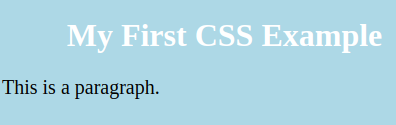
\includegraphics[width=0.97\textwidth]{img/css-example.png}
      \end{block}
      
    \column{0.47\textwidth}

CSS in HTML (\href{https://www.w3schools.com/css/default.asp}{w3s}) -- Darstellung
\begin{htmlcode}
<!DOCTYPE html>
<html>
  <head>
    <style>
body {
  background-color: lightblue;
}
h1 {
  color: white;
  text-align: center;
}
p {
  font-family: verdana;
  font-size: 20px;
}
    </style>
  </head>
  <body>
    <h1>My First CSS Example</h1>
    <p>This is a paragraph.</p>
  </body>
</html>
\end{htmlcode}

  \end{columns}
\end{frame}
%------------------------------------------------------------------------------


\begin{frame}[standout]
  Übung: 
  \begin{enumerate}\small
      \item \alert{\href{https://commonmark.org/help}{Markdown in 60s}} oder 10min Übung
      \item \alert{\href{https://dash.generalassemb.ly/}{HTML / CSS Tutorial (Anmeldung erforderlich)}}
      \item oder HTML/CSS auf \href{https://www.w3schools.com/html/default.asp}{w3s}
      \item \alert{\href{https://latex-ninja.com/2018/12/11/jumpstarting-learn-latex-in-3-minutes/}{\LaTeX{} in 3min} (Overleaf-Anmeldung nötig)}
  \end{enumerate}
\end{frame}



\section{Annotation mit XML}
%-----------------------------------------------------
\begin{frame}{XML: eXtensible Markup Language}
\begin{columns}
\column{0.35\textwidth}
\begin{itemize}\small 
    \item \href{https://www.w3schools.com/xml/default.asp}{W3Schools-Tutorial} 
    \item {Paradigma der Trennung von Form \& Inhalt} 
    \item {XML: Metasprache}
\end{itemize}
\bgupper{w3schools}{black}{.xml} \\

\begin{itemize}\scriptsize 
    \item {RSS}, SOAP, XAML 
    \item {MathML}, {GraphML}~ 
    \item {XHTML}~
    \item {RDF}~
    \item {KML}~ 
    \item {Scalable Vector Graphics (SVG)}
\end{itemize}

\column{0.65\textwidth}
\metroset{block=fill}
\begin{block}{}
\begin{quote}
    Die \textbf{Extensible Markup Language} (dt. \emph{Erweiterbare Auszeichnungssprache}), abgekürzt XML, ist eine Auszeichnungssprache zur Darstellung hierarchisch strukturierter Daten im Format einer Textdatei, die sowohl von Menschen als auch von Maschinen lesbar ist.

XML wird auch für den plattform- und implementationsunabhängigen Austausch von Daten zwischen Computersystemen eingesetzt, insbesondere über das Internet, und wurde vom World Wide Web Consortium (W3C) am 10. Februar 1998 veröffentlicht. \punkti \textbf{XML ist eine Metasprache,} auf deren Basis durch strukturelle und inhaltliche Einschränkungen anwendungsspezifische Sprachen definiert werden. Diese Einschränkungen werden entweder durch eine \textbf{Document Type Description (DTD)} oder durch ein \textbf{XML Schema} ausgedrückt.  (\href{https://de.wikipedia.org/wiki/Extensible\_Markup\_Language}{Wiki})
\end{quote}
\end{block}
\end{columns}

\end{frame}

%-----------------
\begin{frame}{XML-Familie und Vokabularien}
\begin{columns}
\column{0.45\textwidth}
\footnotesize
\bg{w3schools}{white}{XML}~strukturierte Datenbeschreibung \\
\bg{w3schools}{white}{XPath}~Navigation in XMLs \\
\bg{w3schools}{white}{XML Schema}~striktes Datenmodell \\
\bg{w3schools}{white}{XSL}~eXtensible Style Language \\
\bg{w3schools}{white}{XSLT}~Transformation von XML-Dokumenten  \\
\bg{w3schools}{white}{XSL-FO}~ formatierte Ausgabe (z.B. für Druck) \\
\bg{w3schools}{white}{XQuery}~XML-Datenbank-Abfragesprache \\
\bg{w3schools}{white}{und mehr}~
\column{0.45\textwidth}
\metroset{block=fill}
\begin{block}{}
\footnotesize
\begin{itemize}
    \item \textbf{(X)HTML} Hypertext Markup Language 
    \item \textbf{EAD} Encoded Archival Description 
    \item \textbf{TEI} Text Encoding Initiative 
    \item \textbf{CEI} Charters Encoding Initiative (Urkunden)
    \item \textbf{MEI} Music Encoding Initiative 
    \item \textbf{LIDO} Lightweight Information Describing Objects (describing museum or collection objects)
    \item \textbf{SVG} Scalable Vector Graphics 
    \item \textbf{KML} Keyhole Markup Language (Geographie)
    \item \textbf{MathML} 
    \item \textbf{CML} Chemical Markup Language, \dots
\end{itemize}
\end{block}
\end{columns}


\end{frame}


%-----------------------------------------------------
\begin{frame}{XML: eXtensible Markup Language}
\metroset{block=fill}
\begin{columns}
\column{0.45\textwidth}
\footnotesize
\begin{itemize}
    \item deskriptiv $\neq$ prozedural \item erweiterbar (nicht wie bei HTML): kein fixiertes Tag-Set \item UTF-8 kodiert
    \item \bg{alert}{white}{Bedeutung der Daten > Darstellung}
     \item expliziert Implizites oder eine Interpretation \item Hinzufügen von (Meta-)Information \item maschinelle Weiterverarbeitung 
     \item Standard für Beschreibung und Austausch von Daten 
     \item \bg{alert}{white}{universelle Metasprache}
\end{itemize}
\column{0.45\textwidth}
\footnotesize
\begin{block}{}
\bg{w3schools}{white}{Nachteile}~  `geschwätzig', Overlapping-Problem, langsam verglichen mit JSON und relationalen Datenbanken -- hat aber auch Features, die die nicht haben (\& für GeWi sehr wichtig sind)
\medskip

\bg{w3schools}{white}{menschen- und maschinenlesbar}~ 
\medskip

{unabhängig von Ausgabeformat}~ (Papier, Bildschirm)
\end{block}
\end{columns}


\end{frame}

%----------------------------------

\begin{frame}[fragile]{XML-Regeln}
\begin{columns}
\column{0.5\textwidth}
\footnotesize
Prüfung auf \textbf{Wohlgeformtheit} (nach Regeln des XML-Standards) und \textbf{Validität / Gültigkeit} (wohlgeformt \& Schema-Grammatik entsprechend): kann nur geparst werden, wenn wohlgeformt. Schema kann im Notfall ignoriert werden, auch wenn der Validator sich beschwert.

Es gibt Regeln für Elementnamen. Sollen hier nicht im Detail erklärt werden -- Im Zweifelsfall wird man bei der Validierung erfahren, ob man sich einen Fehltritt geleistet hat.
\bigskip

%\includegraphics[width=0.1\textwidth]{doppelkeks.jpg}~\bg{alert}{white}{Doppelkeks} ~ ~\bg{alert}{white}{russische Puppe}~\includegraphics[width=0.15\textwidth]{matroschka.jpg}\vspace{1em}

\mycommand{<key>value</key>}{XML als key-value-Notation} 
\column{0.5\textwidth}\footnotesize
\metroset{block=fill}
\begin{block}{Regeln}
\begin{itemize}
    \item Schachtelung \item genau 1 Wurzelelement (genau 1 äußerste Puppe bei russischen Puppen)
    \item Start- und End-Tag %\item Tagnamen case-sensitive 
    \item leere Elemente erlaubt (\& abkürzbar) \item ordnungsgemäße hierarchische Schachtelung unter Wurzelknoten
\end{itemize}
\end{block}
\bigskip 

\begin{myxml}{Minimalbeispiel}
<?xml version="1.0" ?>
<root>
  <element attribute="value">
    content
  </element>
  <!-- comment -->
</root>
\end{myxml}
\end{columns}

\end{frame}



%------------------------------------------------------------------------------
\begin{frame}[standout]
    \alert{Lektüre}-Zusammenfassung: \\
    DH-Einführung, \emph{XML} \\[1em]
    {\footnotesize Bitte \alert{\href{https://docs.google.com/presentation/d/1JweC-x1MxLjoKcDcHDtsw6NoYZfSbQ0USVYzYxqVx_c/edit?usp=sharing}{hier im Google Slides zusammenfassen}}; 1 Person stellt dann vor. \\
    }
\end{frame}


%---------------------------------------------
\begin{frame}{Trennung von Struktur und Darstellung}

\begin{itemize}
    \item Seit SGML ist ein wichtiges Prinzip die Trennung von Inhalt/Struktur und Darstellung
    \item vermeidet Redundanz, vgl. MS Word `Formatvorlagen': Ich kann das Aussehen des Gesamtdokuments schnell ändern, ohne jede Einzelinstanz umschreiben zu müssen. So auch bei \LaTeX{}, HTML, etc.
    \item der Fokus von XML auf die Beschreibung der Daten erlaubt das \emph{single-source}-Prinzip, d.h. ich kann aus einer Quelldatei, die alle Daten verdichtet enthält, mehrere -- ggf. weniger inhaltsreiche -- auf die Darstellung ausgerichtete Repräsentationen der / Ansichten auf die Daten erstellen (durch eine XSL-Transformation z.B. nach HTML für Webseiten oder \LaTeX{} für den Druck)
\end{itemize}

\end{frame}

